% Copyright 2004 by Till Tantau <tantau@users.sourceforge.net>.
%
% In principle, this file can be redistributed and/or modified under
% the terms of the GNU Public License, version 2.
%
% However, this file is supposed to be a template to be modified
% for your own needs. For this reason, if you use this file as a
% template and not specifically distribute it as part of a another
% package/program, I grant the extra permission to freely copy and
% modify this file as you see fit and even to delete this copyright
% notice. 

\documentclass{beamer}

% There are many different themes available for Beamer. A comprehensive
% list with examples is given here:
% http://deic.uab.es/~iblanes/beamer_gallery/index_by_theme.html
% You can uncomment the themes below if you would like to use a different
% one:
%\usetheme{AnnArbor}
%\usetheme{Antibes}
%\usetheme{Bergen}
%\usetheme{Berkeley}
%\usetheme{Berlin}
%\usetheme{Boadilla}
%\usetheme{boxes}
%\usetheme{CambridgeUS}
%\usetheme{Copenhagen}
%\usetheme{Darmstadt}
%\usetheme{default}
%\usetheme{Frankfurt}
%\usetheme{Goettingen}
%\usetheme{Hannover}
%\usetheme{Ilmenau}
%\usetheme{JuanLesPins}
%\usetheme{Luebeck}
\usetheme{Madrid}
%\usetheme{Malmoe}
%\usetheme{Marburg}
%\usetheme{Montpellier}
%\usetheme{PaloAlto}
%\usetheme{Pittsburgh}
%\usetheme{Rochester}
%\usetheme{Singapore}
%\usetheme{Szeged}
%\usetheme{Warsaw}

\usepackage{ragged2e}
\usepackage{tikz}
%\usepackage{media9}
% Customize Warsaw color 
\setbeamercolor*{palette primary}{use=structure,fg=white,bg=red!50!black}
\setbeamercolor*{palette secondary}{use=structure,fg=white,bg=red!60!black}
\setbeamercolor*{palette tertiary}{use=structure,fg=white,bg=red!70!black}
\part{First Presentation}
% Customize Warsaw block title and background colors
\setbeamertemplate{section in toc}[ball unnumbered]
\setbeamercolor{block title}{bg=red!50!black,fg=white}

\title[Intro to ROS]{Introduction to Robot Operating System (ROS)}


% % A subtitle is optional and this may be deleted
\subtitle{Application to mobile robots}

\author[A.Elhussein]{Amr~Elhussein  \\\and
Advisor: Dr. Suruz Miah}
% - Give the names in the same order as the appear in the paper.
% - Use the \inst{?} command only if the authors have different
%   affiliation.

\institute[Bradley University] % (optional, but mostly needed)
{
  Department of Electrical and Computer Engineering\\
  Bradley University\\
  1501 W. Bradley Avenue\\
  Peoria, IL, 61625, USA
}
% - Use the \inst command only if there are several affiliations.
% - Keep it simple, no one is interested in your street address.

\date[May~31,~2019]{Friday, May~31,~2019}
% - Either use conference name or its abbreviation.
% - Not really informative to the audience, more for people (including
%   yourself) who are reading the slides online

\logo{\hfill\href{http://www.bradley.edu}{
\includegraphics[width=0.75cm]{figs/logoBU1-Print}}}  % place logo in every page 


\subject{Mobile Robot Localization}
% This is only inserted into the PDF information catalog. Can be left
% out. 

% If you have a file called "university-logo-filename.xxx", where xxx
% is a graphic format that can be processed by latex or pdflatex,
% resp., then you can add a logo as follows:

% \pgfdeclareimage[height=0.5cm]{university-logo}{university-logo-filename}
% \logo{\pgfuseimage{university-logo}}

% Delete this, if you do not want the table of contents to pop up at
% the beginning of each subsection:
%\AtBeginSubsection[]
%{
 % \begin{frame}<beamer>{Outline}
  %  \tableofcontents[currentsection,currentsubsection]
  %\end{frame}
%}

% Let's get started
\begin{document}

\begin{frame}
  \titlepage
\end{frame}

\begin{frame}{Outline}
  \tableofcontents
  % You might wish to add the option [pausesections]
\end{frame}

% Section and subsections will appear in the presentation overview
% and table of contents.

\section{Introduction}
\subsection{Historical Background}
\begin{frame}{Intrduction}{History and Legacy}
  
\begin{itemize}
  \item
   Started in 2007 by researches from Stanford AI Robot (Stair) and the Personal Robots (PR) Program and was sponsored by Willow Garage a visionary robotics incubator.
  \item
Used Worlwide in Research and Industry.
  \item
    Currently supported by the Open Source Robotics Foundation.
  \end{itemize}
  \begin{figure}
  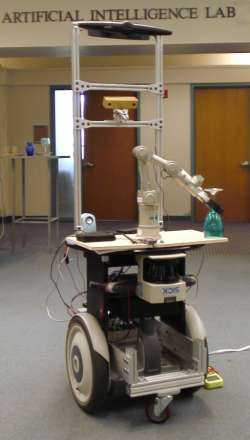
\includegraphics[scale=0.2]{figs/img/stair_small}
  \caption{Stair}
  \end{figure}
  
\end{frame}
\subsection{Robot Programming Before ROS}
\begin{frame}{Intrduction}{Robot Programming Before ROS}
\begin{itemize}
  \item
No common platform for develeoping robotics
  \item
Build every thing from scratch 
  \item
  Algorithm implementation 
  \end{itemize}
  
\end{frame}
\subsection{ROS is ..}
\begin{frame}{Intrduction}{ROS is ..}
\begin{block}{}
 A flexible framework for writing robot software. It is a collection of tools, libraries, and conventions that aim to simplify the task of creating complex and robust robot behavior across a wide variety of robotic platforms.
\end{block}

\end{frame}
%----------------------------------
\subsection{ROS Equation}
\begin{frame}{Intrduction}{Ros Equation}
\begin{figure}
\centering
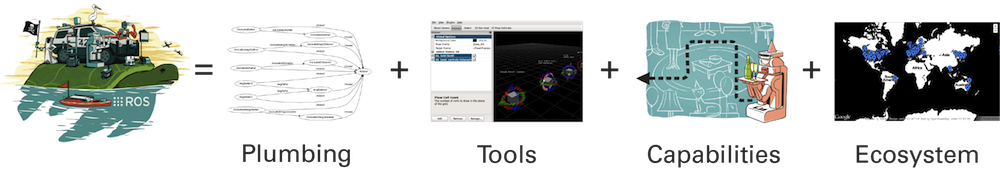
\includegraphics[scale=1.4]{figs/img/ros_equation}
\end{figure}
\end{frame}
%----------------------------------
\subsection{Applications}
\begin{frame}{Intrduction}{Applications}
\begin{figure}
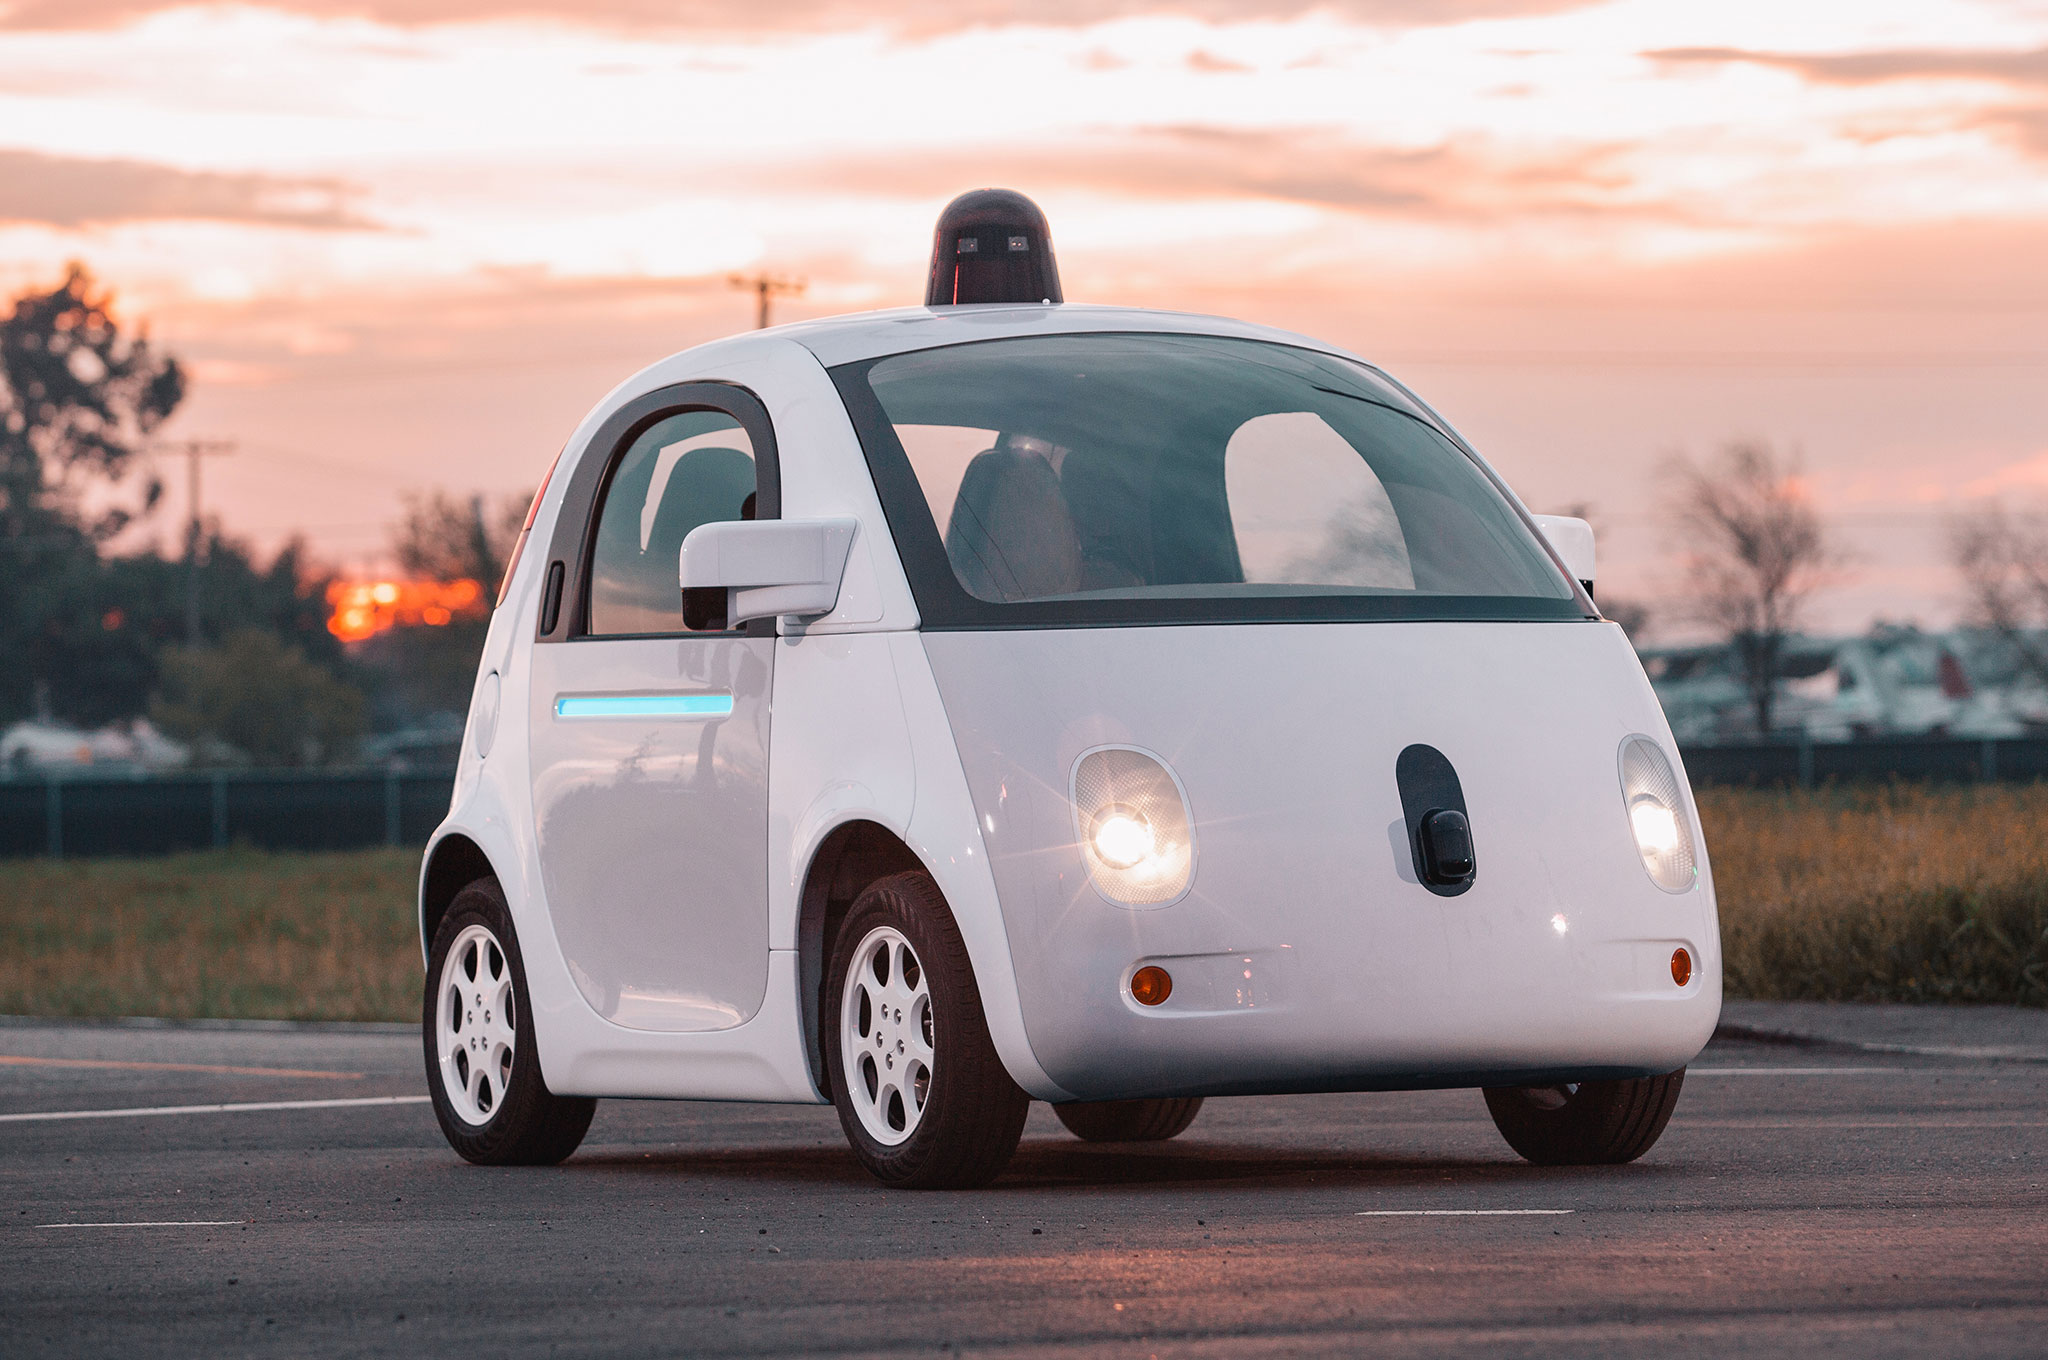
\includegraphics[scale=0.05]{figs/img/selfdrivcar}
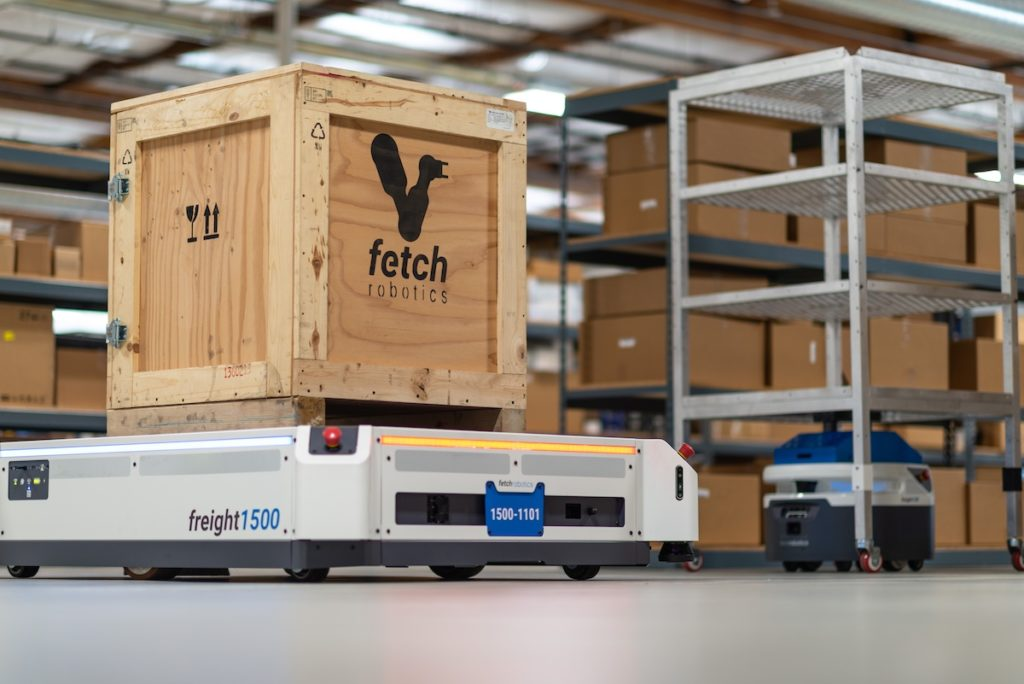
\includegraphics[scale=0.4]{figs/img/warehouse}
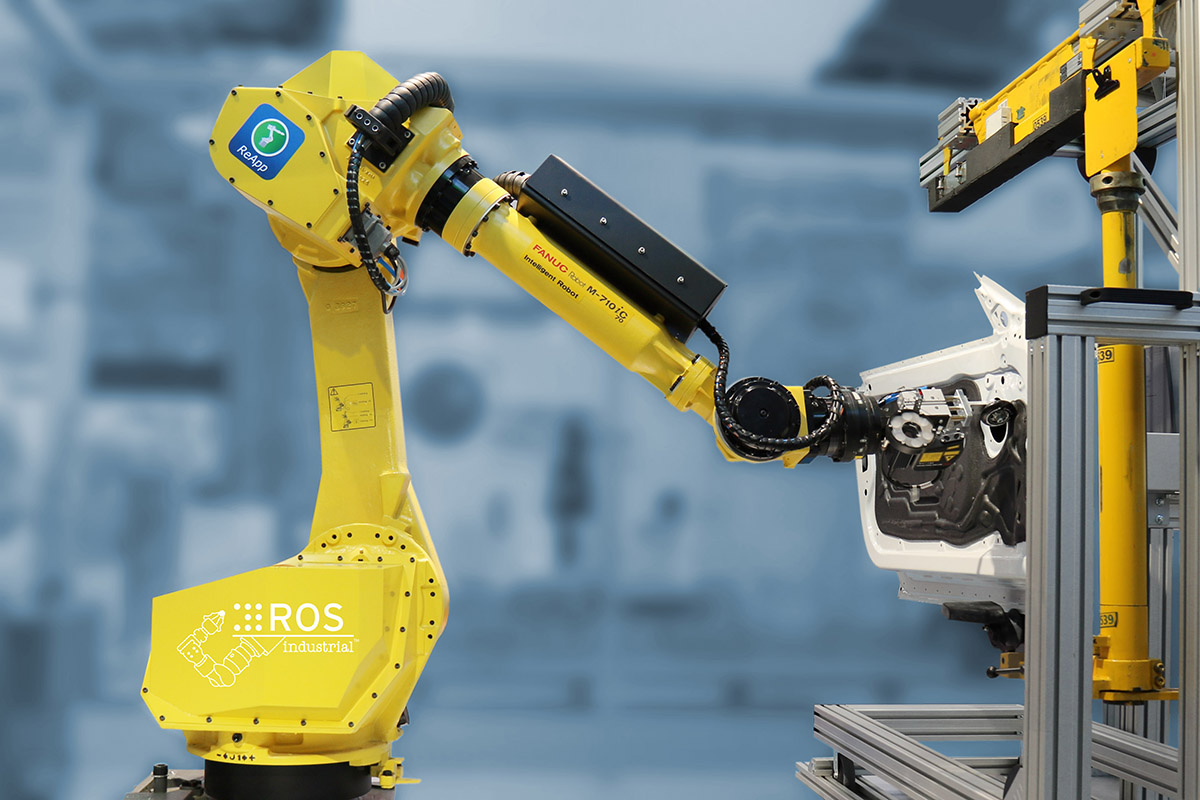
\includegraphics[scale=0.083]{figs/img/industrial}
\end{figure}

\end{frame}
%----------------------------------  



\section{ROS Concepts}

\subsection{Filesystem}

\begin{frame}{ROS Concepts}{Filesystem}
\begin{figure}
\centering
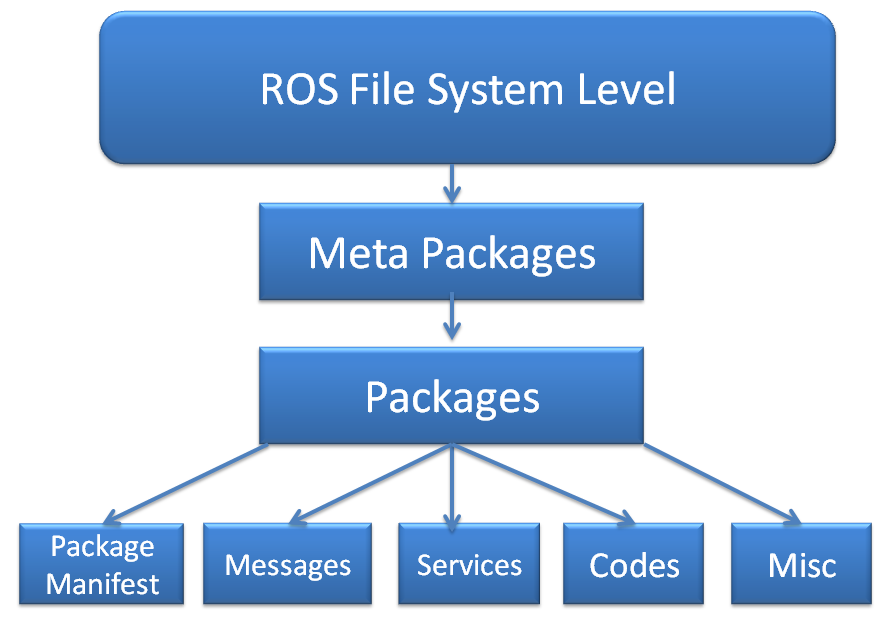
\includegraphics[scale=0.4]{figs/img/filesystem}
\end{figure}
  
\end{frame}

%----------------------------------

\subsection{Computation Graph}

\begin{frame}{ROS Concepts}{Computation Graph}
\begin{figure}
\centering
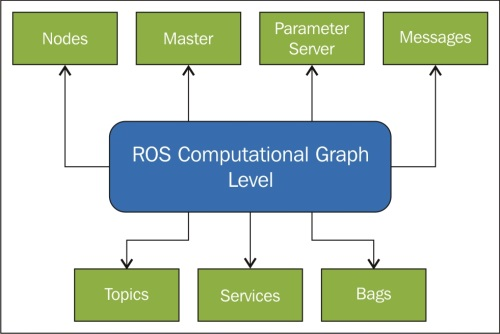
\includegraphics[scale=2]{figs/img/computaiongraph}
\end{figure}
  
\end{frame}
%----------------------------------
\begin{frame}{ROS Concepts}{Computation Graph: Master}
\begin{figure}
\centering
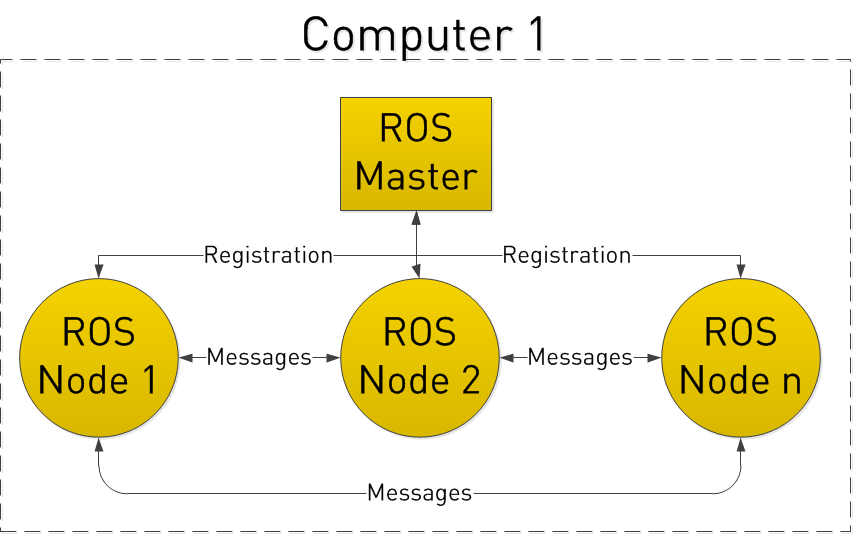
\includegraphics[scale=0.35]{figs/img/master}
\end{figure}

\end{frame}
%----------------------------------
\begin{frame}{ROS Concepts}{Computation Graph: Master}
\begin{figure}
\centering
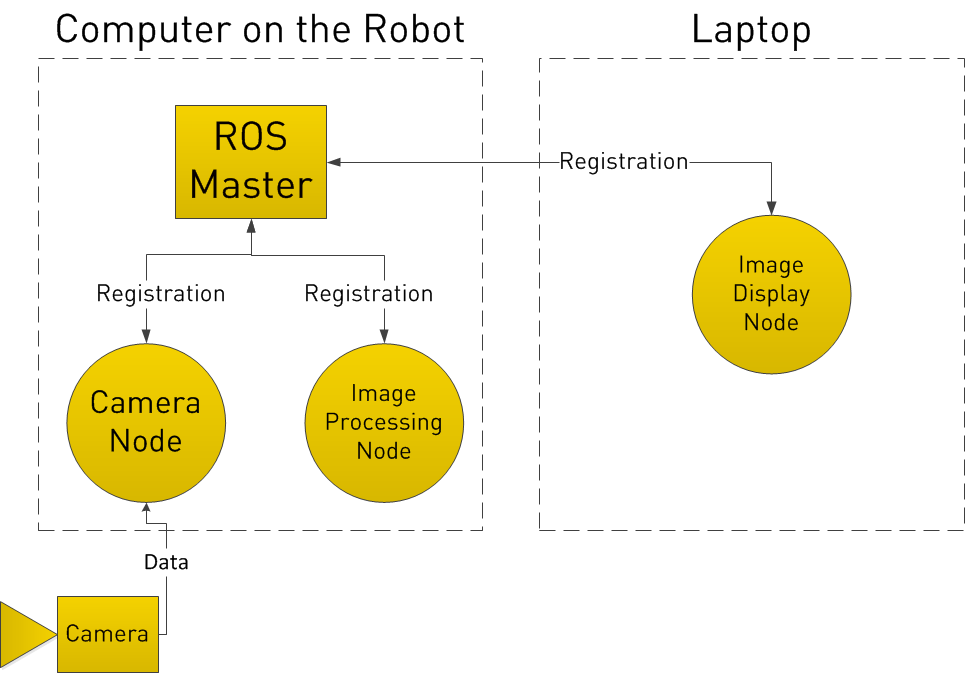
\includegraphics[scale=0.3]{figs/img/nodeseg}
\end{figure}
\end{frame}
%----------------------------------


\subsection{Community level}

\begin{frame}{ROS Concepts}{Community level}
\begin{figure}
\centering
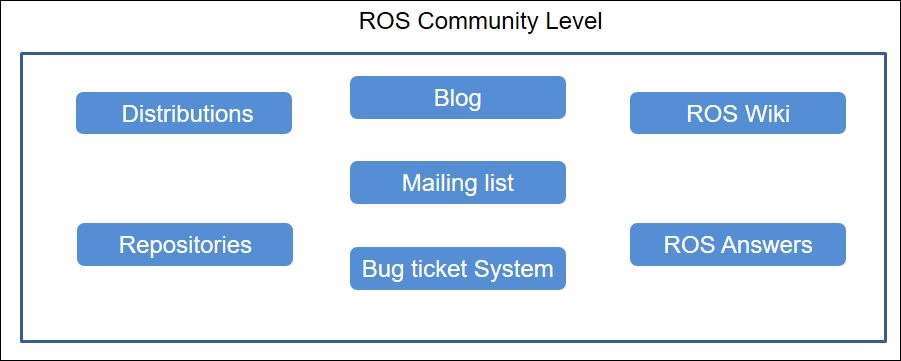
\includegraphics[scale=0.5]{figs/img/community}
\end{figure}
  
\end{frame}

%----------------------------------

\section{ROS installation}
	
\begin{frame}{Installation}

\begin{itemize}
\item Debian-based distributions such as Ubuntu.
\item Many robots.
\item Current supported distributions
\begin{itemize}
\item ROS Kinetic Kame, Released May, 2016.
\item ROS Melodic Morenia, Released May, 2018
%put pics%
\end{itemize}
\end{itemize}

\end{frame}
%----------------------------------
\begin{frame}{Installation}

After choosing the distribution follow the instruction on ROS Wiki which start by:
\begin{itemize}
\item Configure your Ubuntu repositories.
\item Setup your sources.list.
\item Set keys.
\item Install with "sudo apt-get install ros-kinetic-desktop-full".
\end{itemize}

\end{frame}

%----------------------------------

\section{Future of ROS}


\begin{frame}{Future of ROS}

\begin{itemize}
\item Security
\item Critical Missions
\item Distributed Processing
\end{itemize}

\begin{figure}

\includegraphics[scale=0.2]{figs/img/ros2}
\end{figure}  

\end{frame}

%----------------------------------



% You can reveal the parts of a slide one at a time
% with the \pause command:
%\begin{frame}{Second Slide Title}
%  \begin{itemize}
%  \item {
%    First item.
%    \pause % The slide will pause after showing the first item
%  }
  %\item {   
  %  Second item.
 % }
  % You can also specify when the content should appear
  % by using <n->:
 % \item<3-> {
 %   Third item.
 % }
%  \item<4-> {
%    Fourth item.
 % }
  % or you can use the \uncover command to reveal general
  % content (not just \items):
%  \item<5-> {
%    Fifth item. \uncover<6->{Extra text in the fifth item.}
%  }
%  \end{itemize}
%\end{frame}

%\section{Second Main Section}

%\subsection{Another Subsection}

%\begin{frame}{Blocks}
%\begin{block}{Block Title}
%You can also highlight sections of your %presentation in a block, with it's own %title
%\end{block}
%\begin{theorem}
%There are separate environments for %theorems, examples, definitions and proofs.
%\end{theorem}
%\begin{example}
%Here is an example of an example block.
%\end{example}
%\end{frame}

% Placing a * after \section means it will not show in the
% outline or table of contents.
\section*{Questions}
\begin{frame}{}
  \centering \Huge
  \emph{Thanks !}
\end{frame}
%------------------
%New Slides
\part {part 2}
\title{Matlab Robotics Systems Toolbox}
\date[June~4,~2019]{Friday, June~4,~2019}
%\author{Main Author and others}
\begin{frame}
\maketitle
\end{frame}
%---------------------
\begin{frame}{Outline}
  \tableofcontents
  % You might wish to add the option [pausesections]
\end{frame}
%-----------------
\section{Introduction}
\begin{frame}{Introduction}
\begin{block}{According to mathworks.com}
Robotics System Toolbox provides algorithms and hardware connectivity for developing
autonomous robotics applications for aerial and ground vehicles, manipulators, and
humanoid robots. Toolbox algorithms include path planning and path following for
differential drive robots, scan matching, obstacle avoidance, and state estimation. For
manipulator robots, the system toolbox includes algorithms for inverse kinematics,
kinematic constraints, and dynamics using a rigid body tree representation.
\end{block}

\end{frame}
%------------------------
\section{Workflow}
\begin{frame}{Workflow}

\begin{figure}[1]

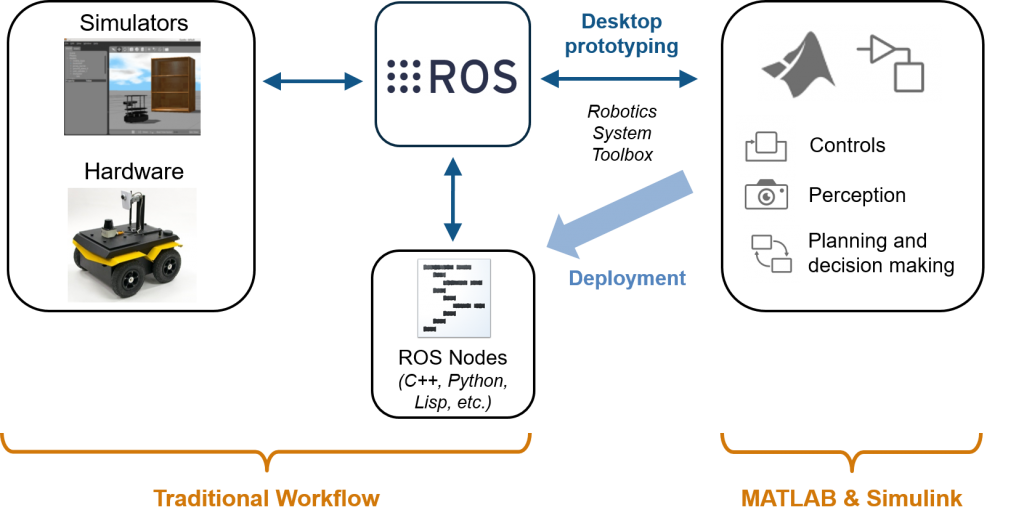
\includegraphics[scale=0.3]{figs/img/matlabworkflow.png}
\caption{Matlab robotics tool box and ROS workflow. courtesy of mathworks.com}
\end{figure}
\end{frame}
\begin{frame}{Workflow}
\begin{figure}
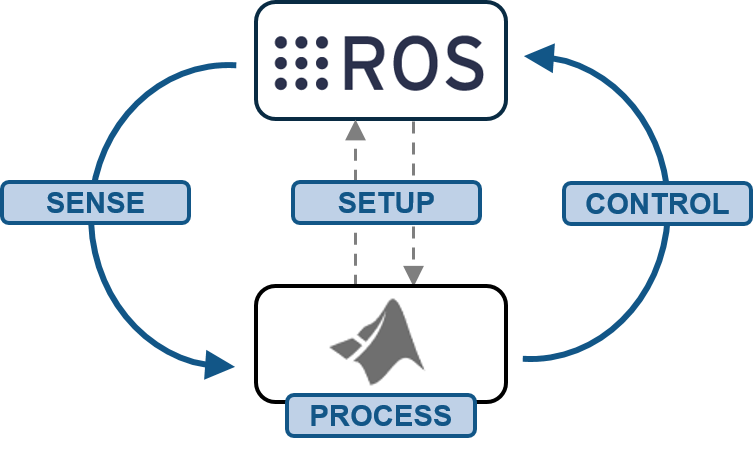
\includegraphics[scale=0.5]{figs/img/matlabros.png}
\caption{Matlab and ROS integration, courtsey of mathworks.com}
\end{figure}

\end{frame}
\subsection{Desktop prototyping}
\begin{frame}{Workflow}{Desktop prototyping}
\begin{figure}
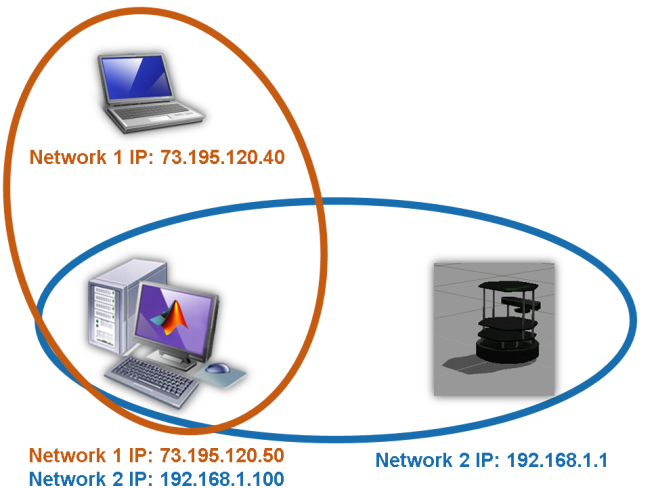
\includegraphics[scale=0.3]{figs/img/desktopproto.png}
\caption{Matlab ROS desktop prototyping, mathworks.com}
\end{figure}
\end{frame}
\begin{frame}{Workflow}{Desktop prototyping}
\begin{figure}
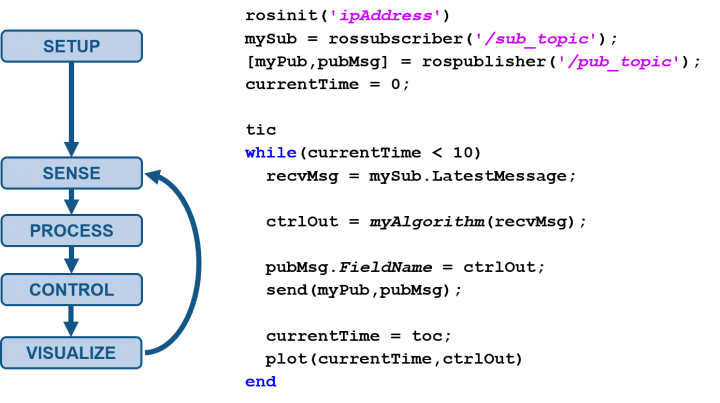
\includegraphics[scale=0.4]{figs/img/desktopproto2.png}
\caption{Desktop prototyping code template, courtsey of mathworks.com}
\end{figure}
\end{frame}
\subsection{Standalone ROS Nodes}
\begin{frame}{Worflow}{Standalone Node}
\begin{figure}
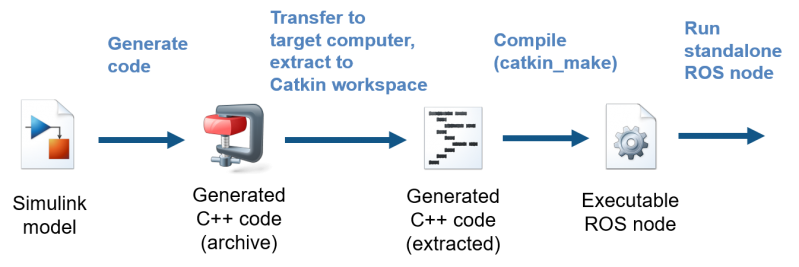
\includegraphics[scale=0.4]{figs/img/rosstandalone.png}
\caption{Generation of ROS standalone node, courtsey of mathworks.com}
\end{figure}
\end{frame}
\begin{frame}{Workflow}{Standalone Node}
\begin{figure}
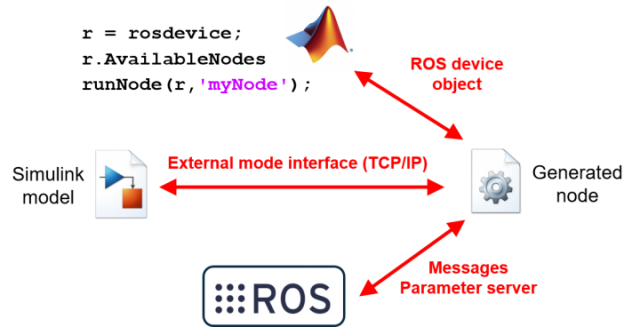
\includegraphics[scale=0.4]{figs/img/rosstandalone2.png}
\caption{Access to ROS standalone node, courtsey of mathworks.com}
\end{figure}
\end{frame}

%---------------
\section{Examples}
\begin{frame}{Examples}
\begin{figure}
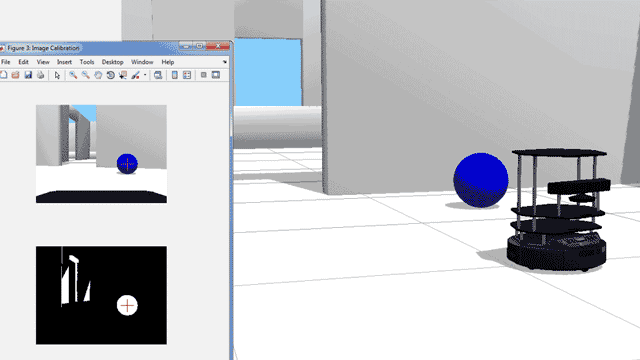
\includegraphics[scale=0.5]{figs/img/turtlebot.png}
\caption{Turtle bot example, courtsey of mathworks.com}
\end{figure}
\end{frame}
%---------------------------------
%New Slides
\part{part 3}
\title{Area Coverage Optimization}
\subtitle{Progress Report}
\date[June~21,~2019]{Friday, June~21,~2019}
%\author{Main Author and others}
\begin{frame}
\maketitle
\end{frame}
%---------------------
\begin{frame}{Outline}
  \tableofcontents
  % You might wish to add the option [pausesections]
\end{frame}
%-----------------
\section{Introduction to V-REP}
\begin{frame}{V-REP}
\begin{columns}
\begin{column}{0.5\textwidth}
General purpose robot simulator with integrated development environment "coppeliarobotics.com".
\end{column}
\begin{column}{0.5\textwidth}  %%<--- here
    \begin{center}
     
\includegraphics[width=0.5\textwidth]{figs/img/vrep.png}
     \end{center}
\end{column}
\end{columns}
\end{frame}
%-------------------------
\section{Interfacing Matlab and ROS on the same Machine}
\begin{frame}{Interfacing}
\begin{figure}
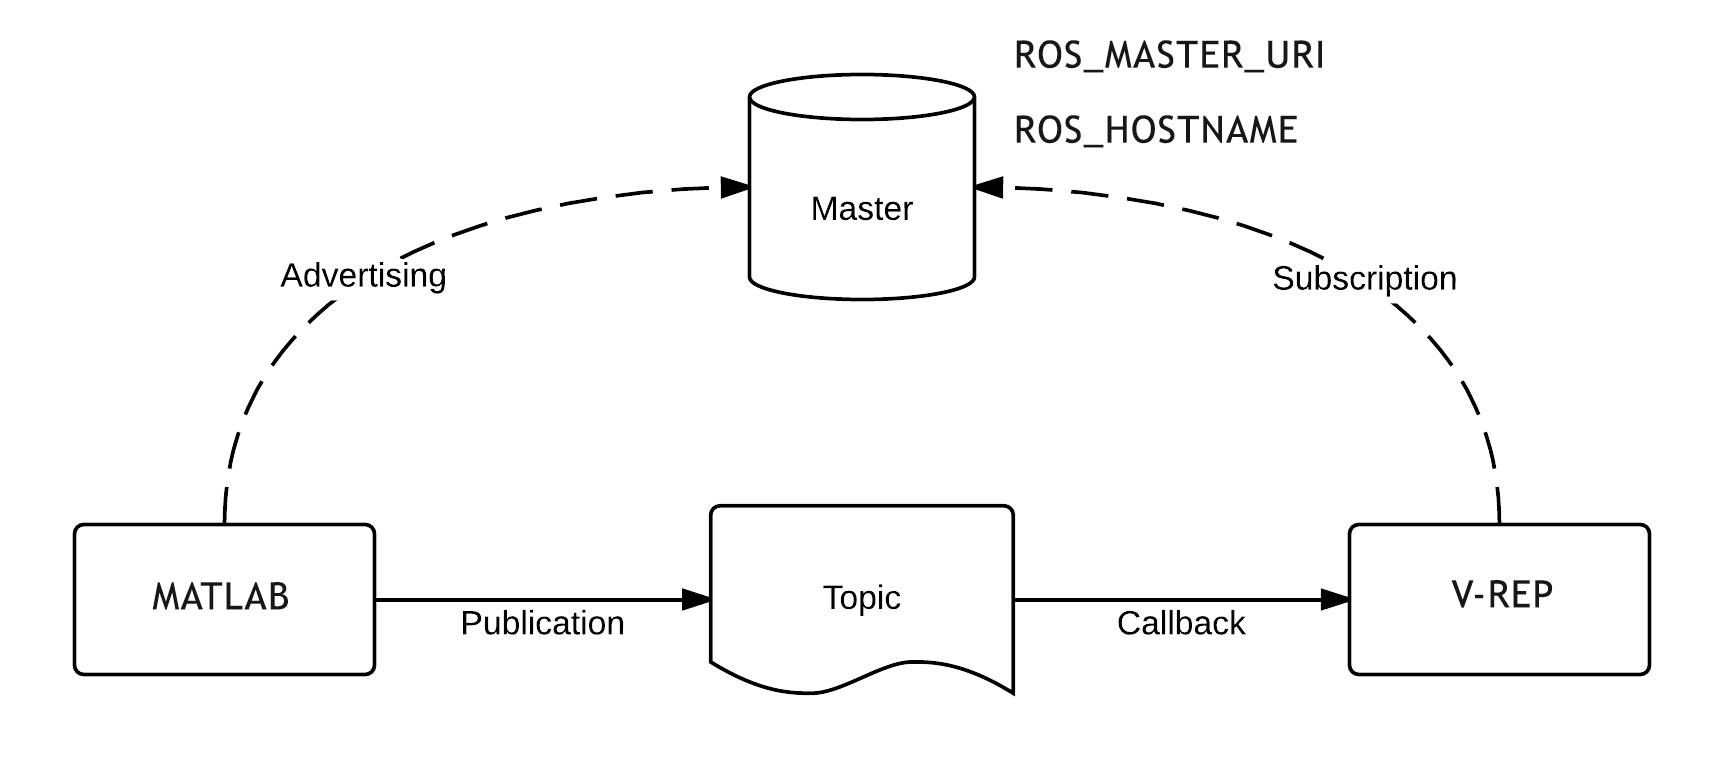
\includegraphics[scale=0.2]{figs/img/interface.jpg}
\caption{ROS, Matlab and V-REP interface}
\end{figure}
\end{frame}
%---------------------------------------
\section{Line following simulation}
\begin{frame}{Line Following}
\begin{center}
\begin{figure}
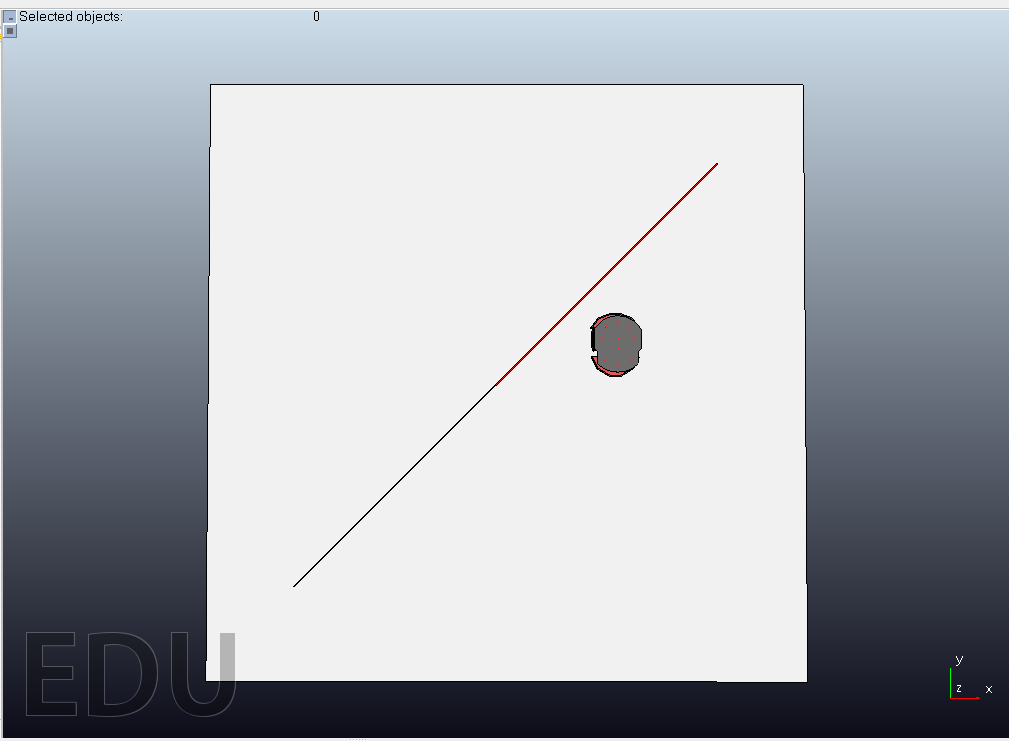
\includegraphics[scale=0.25]{figs/img/line.png}
\caption{Line Following Scene}
\end{figure}
\end{center}

\end{frame}

%---------------------------------------
\section{Leader follower simulation}
\begin{frame}{Leader Following}
\begin{center}
\begin{figure}
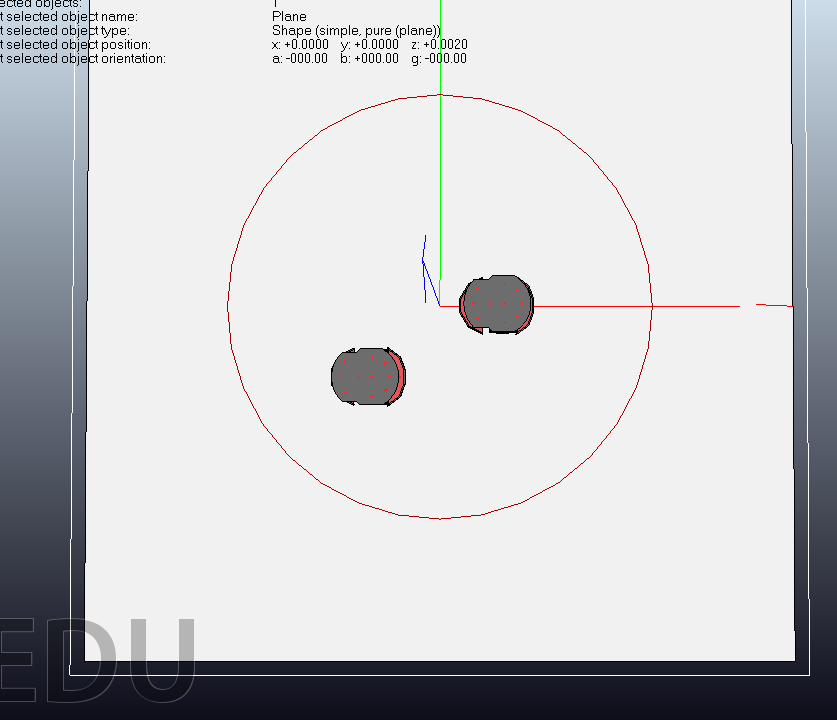
\includegraphics[scale=0.25]{figs/img/leader.png}
\caption{Leader Follower Scene}
\end{figure}
\end{center}

\end{frame}
%--------------------------------------
\section{Area Coverage simulation}
\begin{frame}{Area Coverage}
\begin{center}
\begin{figure}
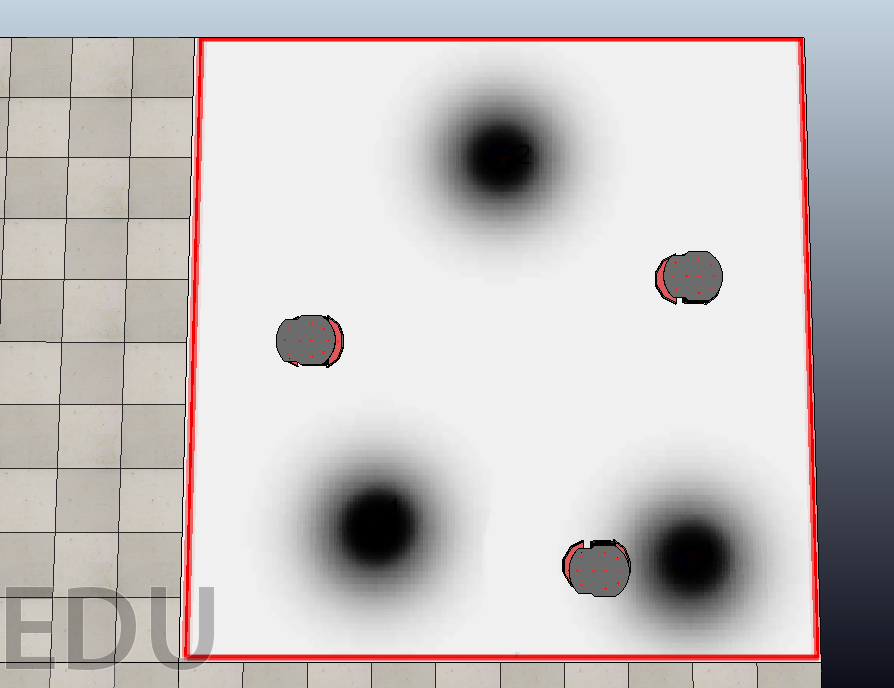
\includegraphics[scale=0.25]{figs/img/area.png}
\caption{Area Coverage Scence}
\end{figure}
\end{center}
\end{frame}
%--------------
\section{Future Work}
\begin{frame}{Future Work}
\begin{itemize}
\item Expiremental Validation.
\item Refining simulation results. 
\end{itemize}
\end{frame}
%----------------------------------
\section*{Questions}
\begin{frame}
\begin{LARGE}
\begin{center}
Questions?
\end{center}
\end{LARGE}
\end{frame}
%---------------------------
%New Slides
\part{part 4}
\title{Area Coverage Optimization}
\subtitle{Progress Report}
\date[July~5,~2019]{Friday, July~5,~2019}
%\author{Main Author and others}
\begin{frame}
\maketitle
\end{frame}
%---------------------
\begin{frame}{Outline}
  \tableofcontents
  \end{frame}
%----------------------
\section{Objectives}
\begin{frame}{Objectives}
\begin{itemize}
\item Refining Simulation
\item Expiremental Validation
\end{itemize}
\end{frame}
%----------------------
\section{Refining Simulation}
\begin{frame}{Refining Simulation}{Modeling}
\begin{center}
\begin{figure}
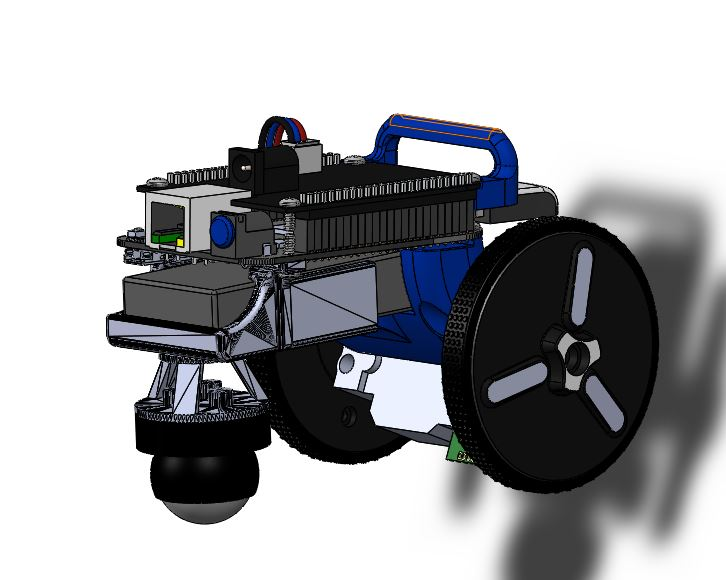
\includegraphics[scale=0.3]{figs/img/solidworks.JPG}
\caption{eduMOD Solidworks model}
\end{figure}
\end{center}
\end{frame}
%-------------
\begin{frame}{Refining Simulation}{importing to V-rep}
\begin{center}
\begin{itemize}
\item Universal Robotic Description Format
\item From Solidworks to URDF
\end{itemize}
\end{center}
\end{frame}
%-------------------------
\section*{Questions}
\begin{frame}
\begin{LARGE}
\begin{center}
Questions?
\end{center}
\end{LARGE}
\end{frame}
%-------------------------------------------
\part{part 4}
\title{Area Coverage Optimization}
\subtitle{Progress Report}
\date[July~19,~2019]{Friday, July~19,~2019}
%\author{Main Author and others}
\begin{frame}
\maketitle
\end{frame}
%---------------------
\begin{frame}{Outline}
  \tableofcontents
  \end{frame}
%----------------------
\section{V-rep simulation}
\begin{frame}{Solidworks to URDF plugin}
\begin{itemize}
\item Tested with simpler models but kept getting the same error
\begin{figure}
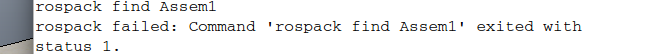
\includegraphics[scale=0.5]{figs/img/error.png}
\end{figure}
\item the error is related to rospack find 
\item testing the urdf file with gazebo and rviz along with windows version of vrep
\end{itemize}
\end{frame}
%----------------------------
\section{Implementation}
\begin{frame}{Implementation}
\begin{itemize}
\item successfully interfacing matlab robotics toolbox with the eduMOD robot through cable and wifi.
\item implemented the line following and leader follower trials and waiting for the recent version of area coverage code to be implemented. 
\item looking deeply into results.



\end{itemize}
\end{frame}
%-------------------------
\section*{Questions}
\begin{frame}
\begin{LARGE}
\begin{center}
Questions?
\end{center}
\end{LARGE}
\end{frame}
%-------------------------------------------
\part{part 5}
\title{Area Coverage Optimization}
\subtitle{Progress Report}
\date[July~19,~2019]{Friday, August~02,~2019}
%\author{Main Author and others}
\begin{frame}
\maketitle
\end{frame}
%----------------------------
\begin{frame}{Outline}
  \tableofcontents
  \end{frame}
%----------------------------
\section{Milestones}
\begin{frame}{Milestones}
\begin{center}
\begin{itemize}
 \item Understand ROS, Matlab robotics Tool box, Vrep,and their interfacing 
 \item Run the simulation demos using pioneer robot and then refining the simulation to get better results 
 \item Understand how to navigate beaglboneblue through ssh
 \item Implement the area coverage algorithm with eduMIP robot
\end{itemize}
\end{center}
\end{frame}
%-------------------------------
\section{Refining simulation}
\begin{frame}{eduMIP urdf}
\begin{center}
\begin{figure}
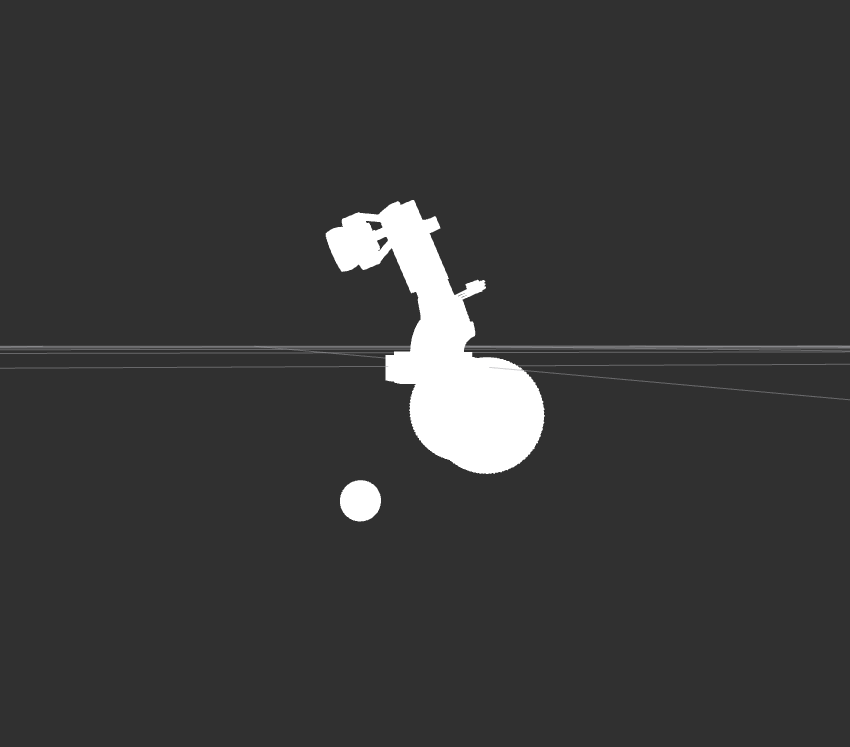
\includegraphics[scale=0.25]{figs/img/rviz.png}
\caption{eduMIP rviz}
\end{figure}
\end{center}
\end{frame}
%--------------------------------
\section{Implementation}
\begin{frame}{Implementation}{line following}
%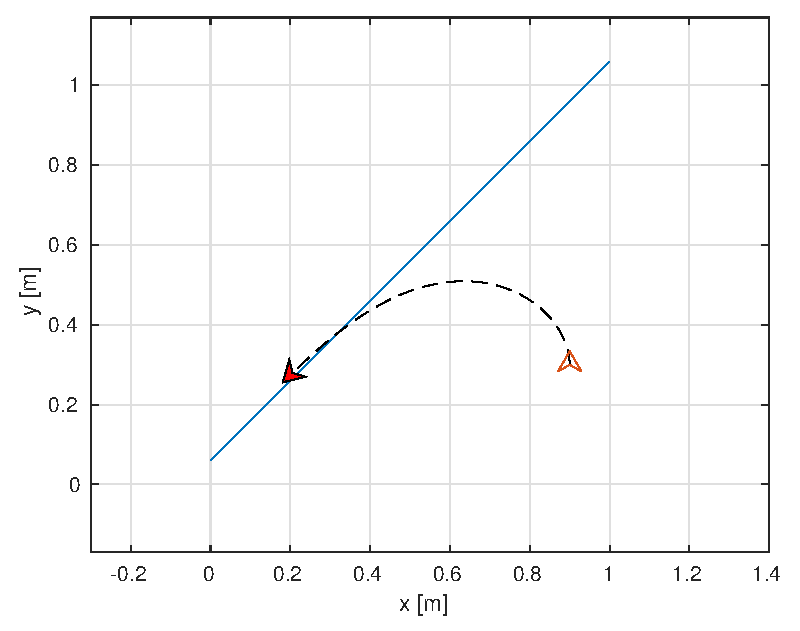
\includegraphics[scale=0.5]{figs/vids/trajectoryLineFollower.eps}
\end{frame}
%----------------------
\begin{frame}{Implementation}{leader follower}
%\includegraphics[scale=•]{•}
\end{frame}
%---------------------
\begin{frame}{Implementation}{area coverage}
\begin{itemize}
\item error in orientation calculation.
\end{itemize}
%\includegraphics[scale=•]{•}
\end{frame}
%-----------------
\section*{Questions}
\begin{frame}
\begin{LARGE}
\begin{center}
Questions?
\end{center}
\end{LARGE}
\end{frame}
%---------------------
\end{document}








